\subsection{Estudiantes Israelíes}

En abril del 2014, 2 estudiantes de ingeniería de software llamados Shir Yadid y Meital Ben-Sinaí del Instituto de Tecnología de Israel, como proyecto de su carrera, crearon su propio software. La función de este software consistía en simular un gran taco en una carretera importante de Israel, para desviar el tráfico por carreteras alternativas, pero teniendo en cuenta que esto podría haber provocado un gran caos fue hecho experimentalmente en una de las calles secundarias de su campus.
Este experimento se compuso de las siguientes etapas según cuentan los estudiantes  ([5],[6]):
\\\\
\begin{itemize}
\item Primera etapa: Crear dispositivos móviles con android falsos con un emulador de android. 
\item Segunda etapa: un sistema de control que simulara la intervención humana en el dispositivo que incluía la creación de una cuenta, iniciar sesión y hacer uso de las funciones de Waze. Esto provocó muchos usuarios “wazers” falsos operando.
\item Tercera etapa: Analizar la densidad del tráfico.
\end{itemize}

Luego de éste trabajo, los estudiantes lo notificaron a los desarrolladores de Waze sobre la vulnerabilidad encontrada.


\subsection{¿Está resuelta esta vulnerabilidad?}

Para comprobarlo, realizamos el mismo ataque. Creando 3 máquinas virtuales con Android 4.4 (aprovechando el proyecto Android X86 [8]) instalamos Waze en cada máquina y realizamos un seguimiento de lo que informa Waze en una misma calle.
\\\\
La instalación de Waze en la máquina virtual fue exitosa y además pudimos verificar la cuenta, pero al momento de cargar el mapa no se pudo, dado al problema de GPS con el cual no se cuenta en la máquina virtual y además alertar en cualquier ubicación fue imposible:



        \begin{figure}[H]
  \begin{center}
    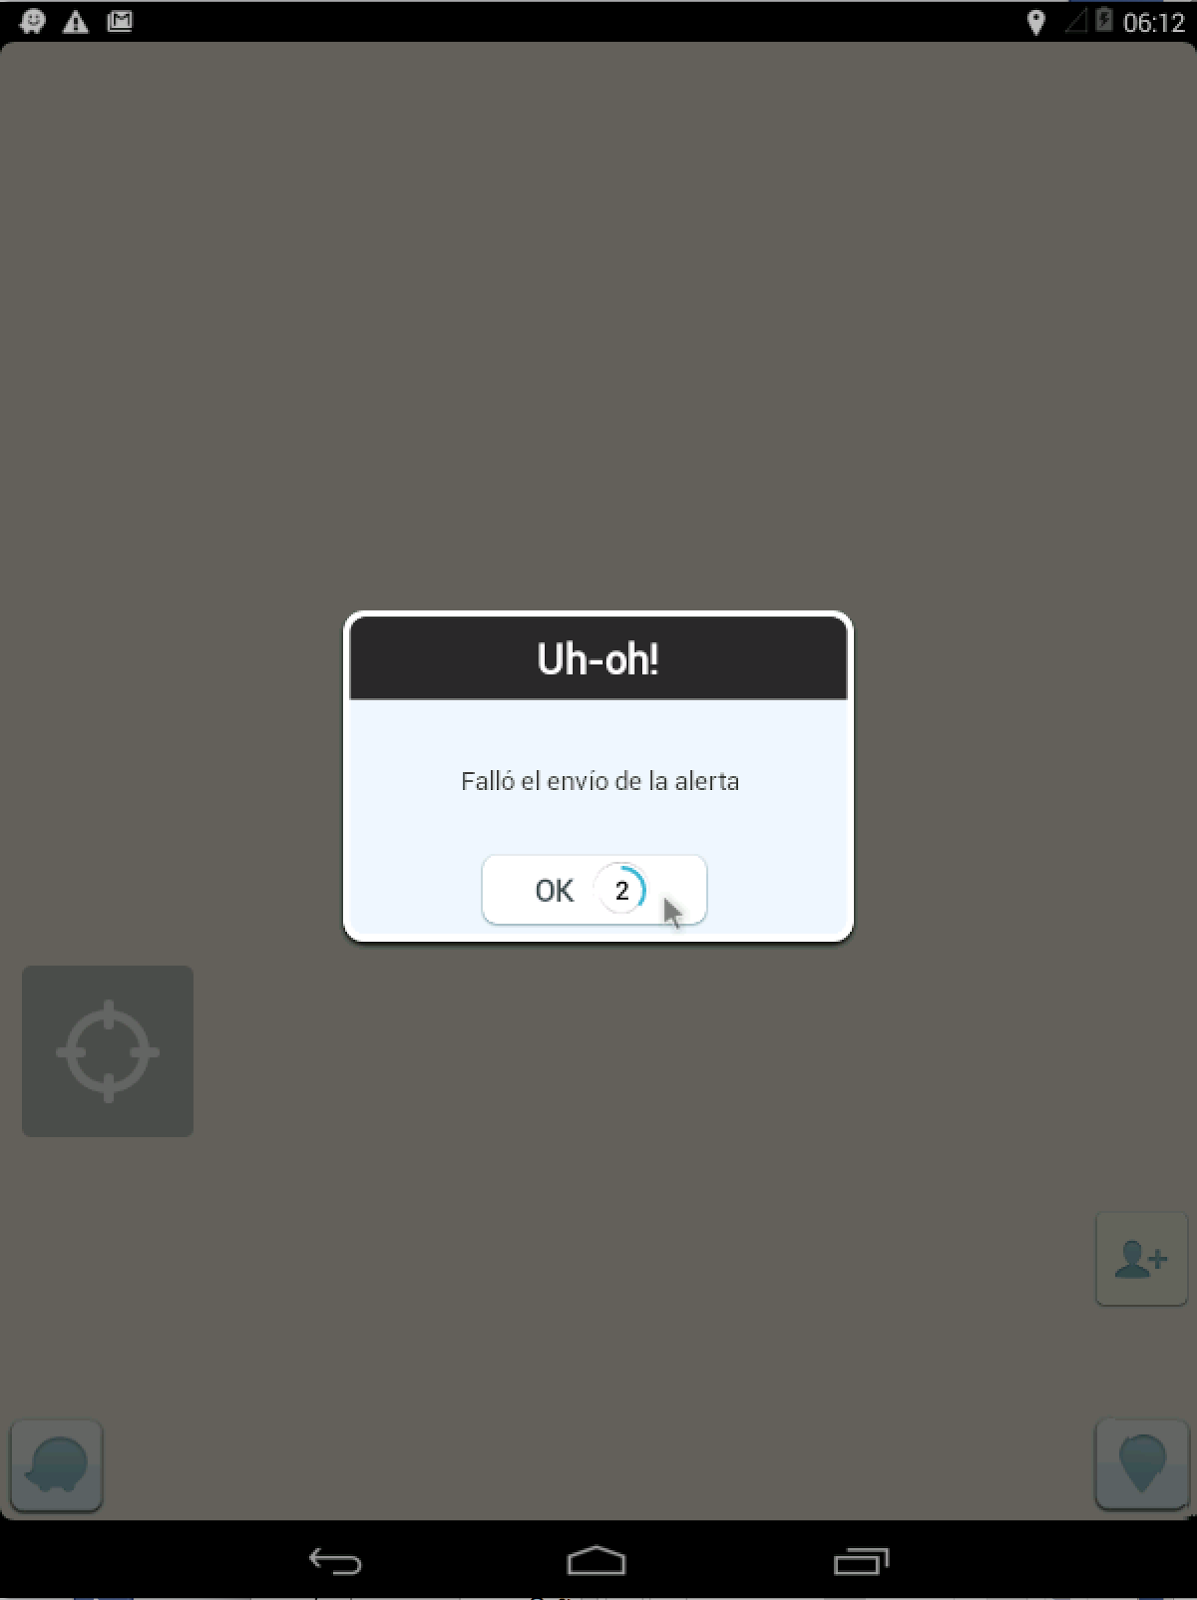
\includegraphics[width=0.4\textwidth]{imagenes/fig18.png}
    \caption{Notificación de Waze de fallo de enviar alerta}
  \end{center}
\end{figure}

Para comprobar si Waze discrimina por información del OS (Android posee un archivo donde guarda la información de la versión del Sistema Operativo), modificamos el archivo /system/build.prop con la misma configuración del teléfono móvil:

    
            \begin{figure}[H]
  \begin{center}
    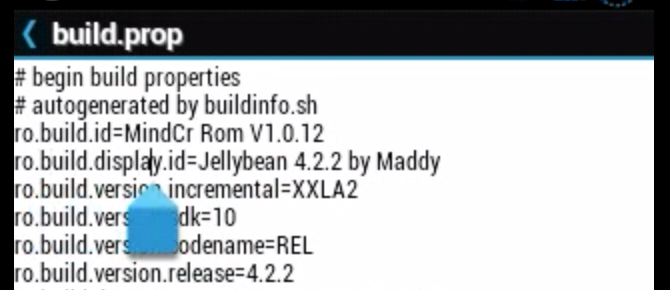
\includegraphics[width=0.9\textwidth]{imagenes/fig19.png}
    \caption{Archivo buld.prop}
  \end{center}
\end{figure}
    
De todas maneras no fue posible enviar una alerta desde una máquina virtual.
\\\\
De manera alterna, se intentó alertar con más de un dispositivo móvil una misma ubicación. Al parecer, si el usuario Waze no ha pasado por la ubicación o no se encuentra cerca, su alerta se recibe pero no se hace válida. En nuestro caso, uno de nosotros desde el sector oriente de Santiago realizó una alerta en el sector sur, La Florida, de tráfico denso. Esta alerta no apareció en la aplicación, pero al alertar cerca de la ubicación apareció inmediatamente en ambos dispositivos.
    
  
    
   \begin{figure}[H]
  \begin{center}
    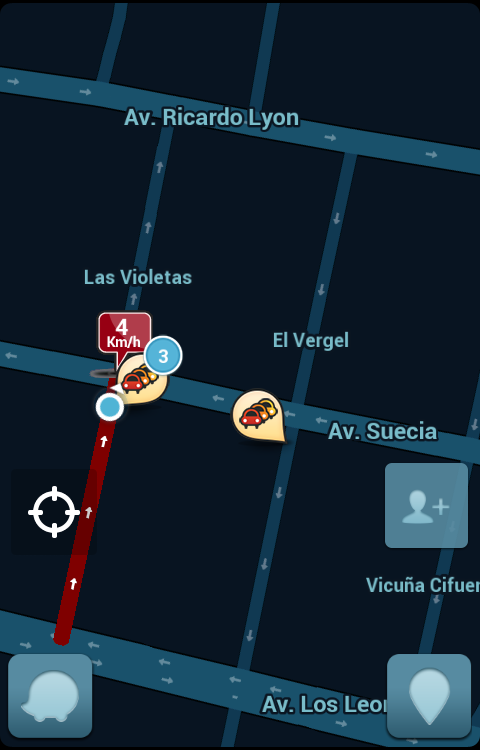
\includegraphics[width=0.5\textwidth]{imagenes/fig20.png}
     \caption{Envío de altertas ubicación 1, dispositivo 1}
  \end{center}
\end{figure}


        \begin{figure}[H]
  \begin{center}
    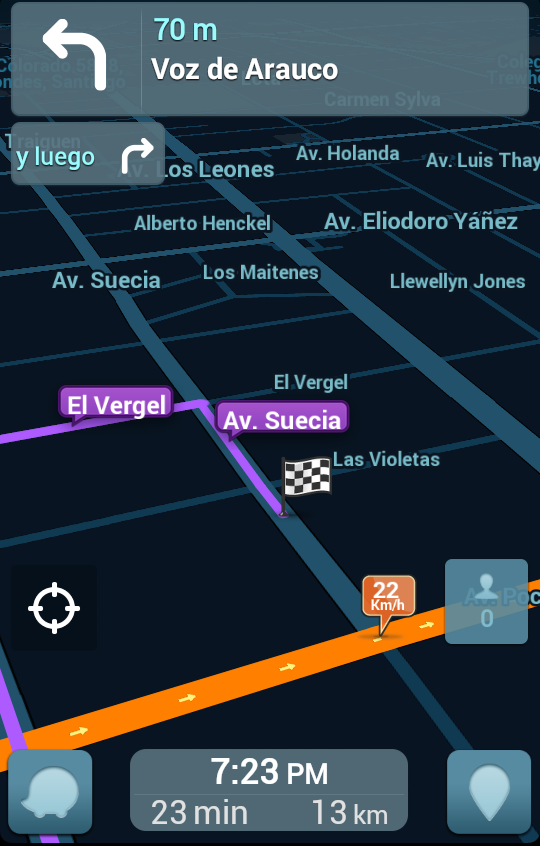
\includegraphics[width=0.5\textwidth]{imagenes/fig21.png}
     \caption{Vista del punnto de envío de las alertas por el dispositivo 1, en el                   dispositivo 2}
  \end{center}
\end{figure}
    
En la figura 11, se muestran 3 envíos seguidos, realizados de alerta de tráfico detenido, desde un dispositivo móvil. Estas alertas fue posible enviarlas por la ubicación del dispositivo, que era cercana a la calle.
\\\\
En la figura 20, desde otro dispositivo no vemos que haya tráfico en la misma dirección.


        \begin{figure}[H]
  \begin{center}
    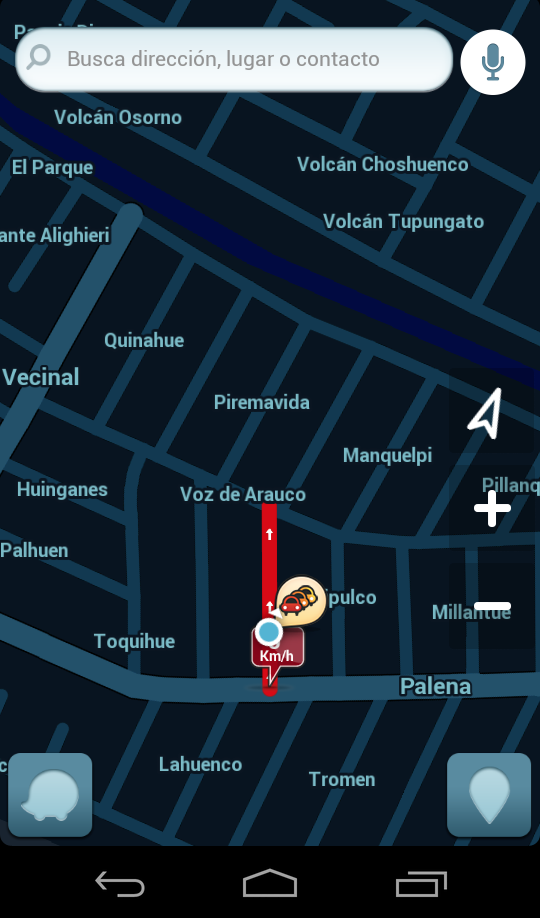
\includegraphics[width=0.5\textwidth]{imagenes/fig22.png}
    \caption{Envíos de alerta en el dispositivo 2}
  \end{center}
\end{figure}


        \begin{figure}[H]
  \begin{center}
    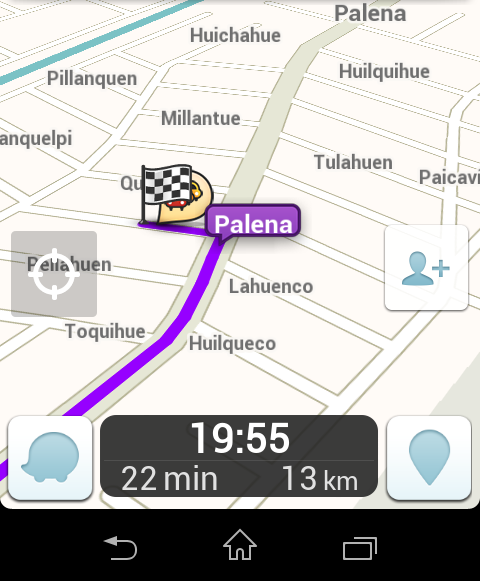
\includegraphics[width=0.5\textwidth]{imagenes/fig23.png}
    \caption{Vista del punnto de envío de las alertas por el dispositivo 2, en el                   dispositivo 1}
  \end{center}
\end{figure}


En caso contrario, usando un usuario frecuente en Waze se hizo la alerta en una calle cercana a la ubicación del dispositivo con ese usuario y con el otro dispositivo si se pudo ver la alerta.
\\\\
En Waze, los usuarios ganan puntos a medida que utilizan la aplicación, a medida que utilizan el mapa, conducen, generan acciones con la aplicación se gana puntaje. [1]
\\\\
Para este ejemplo, el usuario frecuente tiene el ranking de Waze Loyalty, los cuales son los usuarios pertenecientes al 1% de los puntajes más altos de Chile contra un Waze Baby que no ha recorrido más de 100 millas para ascender a otro nivel.
\\\\
Con estas pruebas se comprueba que los desarrolladores de Waze corrigieron la vulnerabilidad encontrada por los estudiantes israelíes.